\documentclass[pageno]{jpaper}

%replace XXX with the submission number you are given from the ISCA submission site.
\newcommand{\IWreport}{2014}

\usepackage[normalem]{ulem}
\usepackage{setspace}
\usepackage{listings}
\usepackage{color}
\usepackage{graphicx}
\usepackage{float}

\restylefloat{figure}
\graphicspath{ {images/} }
\doublespacing

\begin{document}

\title{
SRON: A Coordinated Overlay Network via Software-Defined Networking
}
\date{}
\maketitle

\thispagestyle{empty}

\begin{abstract}

	In this paper, we consider the design and performance of a Software-Defined
Resilient Overlay Network (SRON). While many overlay networks are deployed
on end hosts where they are then configured in a distributed, autonomous
fashion at the ``edge'' of the Internet, our overlay network is run on backbone
switches that support the OpenFlow protocol, and 
whose routing tables are coordinated by a centralized controller.  Running 
an overlay on network switches allows our overlay nodes to route packets with much higher
bandwidth than overlay nodes that run on end hosts, since the hardware in backbone
switches is tailored to routing a large number of packets quickly.  Furthermore, while data forwarded 
over end host overlay nodes must pass through many hops from the Internet backbone to peripheral
end hosts, routing through switch allows data to stay within the backbone, cutting out
several slow hops at the periphery of the network.  The fact that SRON is coordinated by 
a central OpenFlow controller also allows us to use novel probing techniques that would be impossible in a 
distributed overlay; for example, SRON is able to compare the performance of unidirectional 
paths between overlay nodes, whereas in all overlay designs of which the author is aware, only round trip path 
performance is measured.  This centralized controller also means that SRON is able to avoid
generating transient routing loops, since when the controller pushes routing updates to switches, it has 
full knowledge of the routing rules on all switches in the network.
	As SRON is designed to implemented on SDN switches distributed throughout the Internet, we imagine ISPs may use SRON to make more intelligent routing decisions across AS boundaries. 

\end{abstract}

\section{Introduction}

The Internet was designed to be, above all else, scalable. This decision
has allowed it to accommodate billions of users across the world, and central
to this ability is the fact that the Internet is a memory-less, datagram-switching
network. Every router through which a packet passes determines only the next
hop for that packet. As a consequence, however, this lack of central coordination
may lead to sub-optimal routing decisions, and leaves end hosts without control of the
routing of their data.  Central to this limitation is the design of 
the Border Gateway Protocol (BGP), which determines routing between Autonomous
Systems (AS's).  BGP allows Autonomous Systems (AS's) to advertise or hide available routes to one another so as to conform with complex peering contracts between Internet Service Providers.  AS's route via BGP independently of one another, using private route preferences assigned by network administrators in a way that may be financially optimal for the AS but slower for the customers routing data through them.
Andersen, Balakrishnan, Kaashoek, and Morris note that 
``This cost arises because BGP hides many topological details in the interest of
scalability and policy enforcement, has little information about traffic conditions,
and damps routing updates when potential problems arise to prevent large-scale
oscillations''\cite{ron}.  

An overlay network, however, can often make better routing decisions than those of BGP.
In an overlay network, a set of network nodes (which may consist of, for example, end hosts running 
an application-level overlay program) chooses to route data {\it on top} 
of the existing Internet by imagining each node in the overlay connected by ``virtual links''.  These virtual
links may consist of hops over several physical links, with routing between nodes determined natively by
Internet routers.  The overlay allows for faster routing than the Internet when the direct path between
two nodes in the overlay is slower than a two-virtual-link hop path through nodes in the overlay (i.e. when 
routing through an intermediary overlay node is faster than routing between the two nodes directly).
Andersen et al. at MIT leveraged this fact when they created RON\cite{ron}, a 
``Resilient Overlay Network''.  RON consisted of software running on several end 
hosts distributed throughout the Internet, working
together to decide how packets should be routed through the nodes and links in this
overlay. As a result, nodes in RON were able to communicate despite outages 
must faster than hosts routing through the Internet alone.

While a significant body of work addresses the design of such resilient overlays,
none known to this author to date considers an overlay network implemented in a 
Software-Defined Network (SDN).  An SDN overlay presents several advantages over a 
distributed, end host overlay.  For example, the existence of a centralized SDN
controller in an overlay network means routing decisions can be made by an entity 
with a holistic view of the nodes in the overlay, and thus more intelligently than 
routing decisions made by distributed end hosts.  Furthermore, overlays implemented on
switches within the Internet backbone are able to route packets much more quickly and in
higher quantity than end hosts at the periphery of the Internet.

SRON is such a Software-Defined Overlay.  We envision it being used by Internet Service
Providers who wish to route more efficiently between their routers and switches that
may be scattered widely across the Internet and connected to each other through various
other ISP's.  

\section{Past Work}

\subsection{Wide-Scale Internet Performance}
BGP is the path selection algorithm used by backbone Internet routers to make 
decisions about routing between Autonomous Systems.
Interior gateway protocols or IGP's, on the other hand, are routing algorithms used by individual
AS's to decide paths within the AS. IGP's like the frequently-used OSPF\cite{ospfrfc}--a shortest-path link
state routing protocol--determine paths by examining link performance and least
number of hops.  While AS's may be motivated to route packets to customers most 
efficiently when communication is within their domain, business concerns play a 
significant role in determining BGP's ``policy'' routing decisions; that is, BGP
allows AS's to hide routes from other AS's if, for example, the two AS's do not have
an explicit agreement to share infrastructure.  Furthermore, an AS may choose to 
pass a client's data to another AS so that it has more capacity on its infrastructure,
even if such a path is sub-optimal.  Varadhan, Govindan, and Estrin proved that BGP
policies may not even lead to routing convergence--that is, AS's may choose to 
route in such a way that leads to persistent oscillations\cite{varadhan}.  Labovitz et al.\cite{labovitz}
conducted a two year study of Internet routing convergence and found router may take tens of minutes to converge after a fault due to BGP's routing table oscillations. 

\subsection{Overlay Networks}
Overlay networks have been deployed to support several applications that the Internet
alone cannot; for example, Content Distribution Networks (CDN's) are overlays that 
dynamically cache content across the Internet and deliver it to end users to avoid congestion.
Today, CDN's make up the bulk of overlay traffic\cite{kurian}.\bigskip
IP multicast--the method of sending a single packet to multiple receivers in a single transmission--has also been cited as a promising application of overlays.  IP multicast makes applications with multiple receivers more efficient, but is difficult to deploy and today is mostly implemented within a single domain rather than spanning multiple domains\cite{kurian}.  MBone\cite{Macedonia:1994:MPA:618987.620017} was an early overlay that attempted to connect multicast domains by using IP tunneling to transport data across domain boundaries.  Unfortunately, MBone experienced unreliability, heavy loss, and low throughput\cite{kurian}.  Narada\cite{Banerjee:2002:SAL:964725.633045} was proposed as an application-layer alternative to IP multicast, in which overlay nodes created their own routing mesh atop the Internet and serviced multicast in this way.\bigskip
Another important application of overlay networks is end-to-end performance and resiliency; The Detour\cite{Savage:1999:DII:623285.624244} overlay used 45 distributed servers to probe paths between them using the traceroute program; they were curious to know whether or not data could be routed from points A to B more efficiently by routing data through one of their overlay nodes C (i.e. could they choose faster routing paths than the Internet natively).  For roughly half of the paths they measured, they found an alternative route which was faster.  RON\cite{ron} was an overlay network that, inspired by the findings of Detour, used frequent probing in combination with link state routing to find low-latency or high-bandwidth paths between overlay nodes.  RON was implemented as on end hosts, and these overlay nodes were arranged in a fully connected mesh.  The fact that RON was fully connected--each of RON's $n$ nodes had $(n-1)$ neighbors--and used frequent probing meant that it could not (and was not intended to) scale beyond about fifty nodes.  However, a 12 node RON overlay was still able to overcome almost all routing outages in under twenty seconds.
Later modifications to the basic RON design allowed for overlay networks that could find paths with similar performance to RON nodes with much less probing.  One of the most interesting of such techniques which is quite similar to the probing design of SRON is work by Gummadi et al.\cite{Gummadi:2004:IRI:1251254.1251267}; in this mesh, routing is done as follows: when a node at $A$ wants to send data to $B$, it randomly chooses $k$ nodes in the overlay and routes through them; it then uses the intermediary with the first response to route all subsequent packets, and if at any time this path becomes unresponsive, it chooses a second random $k$ nodes and tries again.  They found that $k=4$ gives near maximum benefits. 


\subsection{Software-Defined Networking}
SRON is implemented on a Software-Defined Network--that is, a network on which routers and switches are programmable, and whose routing rules can be updated dynamically from an SDN controller.  In SDN, the {\it control plane}, which makes decisions about how traffic should be handled, is separated from the {\it data plane}, which itself forwards the traffic\cite{Feamster:2014:RSI:2602204.2602219}.  The control plane is embodied by an SDN controller which communicates with network switches and routers in the data plane via an API.  In SRON, we use a popular API known as OpenFlow\cite{McKeown:2008:OEI:1355734.1355746}, a protocol supported by most major switch vendors.  


{\bf Motivations}\bigskip


\subsection{SRON: A Software-Defined Approach}


In the past, overlay networks have been deployed on end hosts and coordinated 
in a distributed fashion.  Indeed this was a natural choice, since users of 
overlay networks were often individuals scarcely located throughout the Internet--
for example, users of the Tor Network (awkward).  A more centralized control
would require not only coordination amongst network users but also would likely have 
significant bandwidth overhead.  If an overlay need be coordinated by a single entity,
then there would have to be some efficient method of communication with that coordinator, but 
finding efficient routes between overlay nodes is exactly the problem that overlay networks are designed to solve--a chicken-and-egg problem.  

{\bf SRON runs on a controller + switches}\bigskip

In SRON, we consider a different application of overlay networks. Like a typical overlay,
SRON consists of nodes that probe each other to determine link latencies, but these nodes
are network switches rather than end hosts. Furthermore, a central SDN controller coordinates 
the probing and routing rules of the switches in the network. 

At first blush, one might 
wonder why an overlay network is necessary on a Software-Defined Network. After all, generally
these networks are deployed by organizations that have entire control over the links in the 
network (for example, a university network, or Google's private backbone). However, we imainge
SRON being deployed on the networks of Internet providers that may span the globe, and who may
need to pass data across other ISPs. In this case, we imagine that the network controller is 
distributed, and the switches is controls are scattered across the globe. The links between 
our switches are not physical links, but a sequence of hops across the Internet. Some of the 
nodes in the multi hop paths between switches may belong to the ISP deploying the overlay, 
but others may be managed by other ISPs.  Thus the SRON overlay network model assumes that all
nodes within it are fully connected, but that the links between them have varying performance 
characteristics.\bigskip

{\bf Advantages of SRON over RON}
Why is such a Software-Defined overlay useful? RON\cite{ron} showed that overlay networks can 
perform significantly better than the raw Internet in terms of overcoming routing outages. That 
being said, routing packets on end hosts has several disadvantages; for one, end hosts are 
much slower at routing data than network switches, whose hardware is custom-tailored for this task.
Second, because routing is done in a hierarchal fashion in the Internet, packets must pass 
through many more hops to get to an end host (that is at the periphery of the Internet) than a 
network switch.
{\bf This part is really questionable:} 
For example, suppose a host in the Computer Science Department at Princeton 
were running an overlay node. While there is likely only a single Cisco switch allocated to all of 
Princeton, a packet destined to be routed through our host node would have to pass first through this 
switch, then through Princeton's University switches, then through the Computer Science Department
routers, and back again.


\section{Design of SRON}

\subsection{Probing Scheme}

\begin{figure}
{\bf SRON Deployment}
\centering
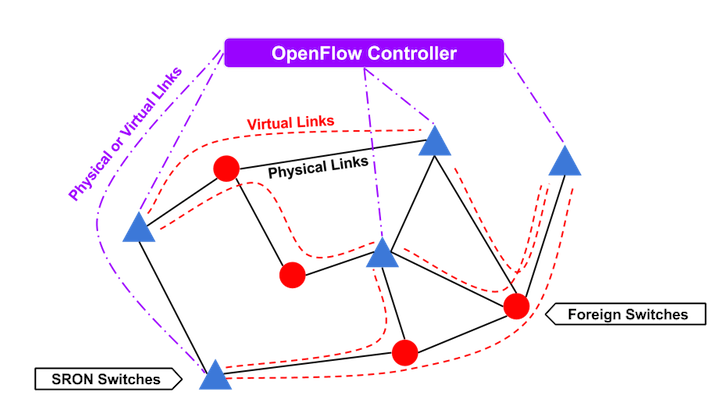
\includegraphics[scale=0.7]{sron.png}
\caption{Here, the triangles denote routers and switches in SRON, which we can program via an OpenFlow controller.  SRON switches may be distributed throughout the Internet and connect to each other via other switches that are not within the same ISP's domain; these ``foreign'' switches that are not controlled by the SRON controller are displayed as circles; SRON nodes are connected in a clique topology via virtual links that may be comprised of multiple hops over physical links, as denoted by the dashed line in this figure.  The connections between the SRON controller and switches may be direct, physical links or virtual links.}
\end{figure}

In SRON, our goal is to measure the latency on the virtual links between nodes and make reactionary
routing decisions. Here we say ``virtual'' because these links may consist of a sequence of hops
across switches and routers in the Internet. At first, the problem of measuring link latency 
might seem straightforward--send a packet between two switches in the network and measure the time
it takes to get between them. Unfortunately, this is not so simple; for one, it is almost impossible
for two nodes in the Internet to measure one-way trip time, since we cannot assume clocks on these
nodes are synchronized (and so packets can't be timestamped). While we can measure path round trip 
time (RTT), there may be a large disparity the latency on either half of the path (indeed, asymmetric
paths is a common consequence of policy routing via BGP). Thus if we were to use RTT as an indication 
of the performance of a link, we may find that ignore a fast link when RTT is high but only one direction
of the connection is slow, or prefer a slow link when RTT is low due to one direction of the connection
being fast. 

An alternative approach we might consider in a software-defined network is to have the network controller 
instruct switch A to send a packet or ``probe'' to switch B, and have switch B pass the packet back 
to the controller. This probe packet may be marked with a distinguished IP address, $PROBEIP$, to allow
switches to treat it as a probe rather than normal network traffic. 
Since the controller is connected to either probe, it can measure the time it takes 
for a packet to get from the controller to switch A to switch B and back again.  This avoids the problem 
of measuring round-trip time from A to B, but is only a valid measurement if the path between controller 
and switches is short compared to the time it takes for a packet to travel from A to B. Since the 
controller-switch connection is likely to run over the Internet, though, we do not believe this would be 
a valid measure of the latency between A and B because the time it takes for a packet to get from the controller
to either of these switches may well rival that of the path time between switches.

\begin{figure}
{\bf Switch Rules for Handling Probes }
\centering
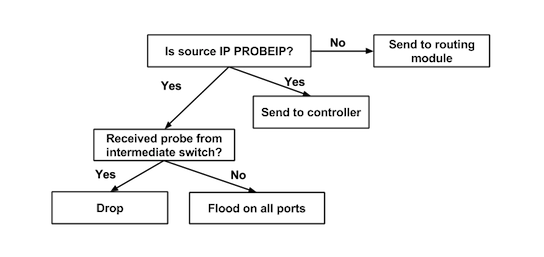
\includegraphics[scale=0.7]{probeHandler.png}
\caption{If a switch receives a probe with the source IP address $PROBEIP$, it sends the probe to be logged at the controller; furthermore, if this switch is the first hop in the probe's path--determined by the destination IP of the probe--then the switch forwards it on all ports.  Otherwise, if this switch is the second hop, it drops the probe.}
\end{figure}


Our measurement of link performance in SRON is somewhat novel in that it does not attempt to calculate 
the time taken along virtual links in the network, but evaluates routes only by their relative performance 
to other routes. For example, a path $p$ from $Switch_A$ to $Switch_B$ is ``better'' than path $p'$ from 
$Switch_A$ to $Switch_B$ if packets sent from $A$ along $p$ reach $B$ faster than those sent from $A$ along
$p'$.  In SRON, we do this by sending probes along all single and double hop paths from $A$ to $B$.
Recall that SRON runs on a clique topology, where every SRON node is connected to every other SRON node.
To determine the best path from $Switch_A$ to $Switch_B$, we have the controller inject probe packets--packets with
designed source IP addresses $PROBEIP$--to $Switch_A$.  These packets are also given a special destination
IP address that denotes that this probe packet originated from $Switch_A$. $Switch_A$ is instructed by 
the controller to forward these probe packets over all ports connected to other switches in the network. 
When a second switch, $Switch_C$, receives such a packet, it recognizes it as a probe by checking that 
the source IP is $PROBEIP$, and sends the packet up to the controller. This probe gives the controller 
information about the performance of the direct path between $Switch_A$ and $Switch_B$. We would also 
like to know about the performance of paths originating at $Switch_A$ that use $Switch_C$ as an intermediate
hop. Thus, if $Switch_C$ finds that it received this probe directly from $Switch_A$--it does this by 
comparing the destination IP address of the probe to the port on which it received this probe--it 
floods the probe on all ports that are not connected to $Switch_A$. Thus eventually $Switch_B$ will
receive a probe originating at $Switch_A$ but passing through $Switch_C$ (since the network is a 
clique), and will send this packet up to the controller. Thus the controller has knowledge about all
single and two-hop paths from $Switch_A$ to $Switch_B$, and knows their ordering by comparing the 
order in which it received probes amongst all paths. Evaluating routes in this way is convenient 
because it allows us to 
\begin{enumerate}
\item
The way probing is actually done in SRON -> on a timer, ever switch sends a probe to every other probe,
forwards once, sort of like multicast tree
\item
Controller keeps track of best route, and stores data about how long this has been this best route (i.e.
stores history so that it can change if a compelling better route appears) 
\end{enumerate}

\subsection{Migrating Routes}

How does the controller decide when to update flow rules between to switches in the network?  On one hand,
if $Switch_A$ sends to $Switch_B$ through $link_1$ but we find that $link_2$ is a significantly faster 
route, we would certainly like to update $Switch_A$'s path to $Switch_B$ in $Switch_A$'s flow table. What do we mean,
though, by ``significantly'' faster?  Not only does it take time to push rule updates to the switch flow tables,
but switching too frequently may cause routing ``oscillations''--that is, flow rules are updated so frequently 
that they cause routing loops, and so no data can pass through the network! For example, if $Switch_A$ decides 
to route to $Switch_C$ through $Switch_B$, and then $Switch_A$ chooses a different route to $Switch_C$ but then
$Switch_B$ decides to route to $Switch_C$ through $Switch_A$, and so on, a data packet may be caught in a routing
loop between $Switch_A$ and $Switch_B$. Finally, Internet protocols such as TCP assume that data travels over
more or less the same path between hosts in the network (this is a crucial component of its congestion control 
mechanism), and so frequent routing changes may render this technique ineffective. Thus we need to set a threshold
for when we decide to migrate routes, and should also keep a history of the performance of different routes so that
our updating mechanism is robust against short fluctuations in route performance. 

We do this as follows:
For each pair of switches, we keep a history of the performance of probes that have taken different paths between
those two switches. For example, for $Switch_A$ and $Switch_B$, we calculate a metric for each path between them--
the direct route between $Switch_A$ and $Switch_B$ as well as the route from $A$ to $B$ through $C$, $A$ to $B$ 
through $D$, and so on. Here is how we calculate the metric of a path $p$ with sequence number $n$: a probe 
is sent along every path from $A$ to $B$ and each probe arrives at the controller in some order. Suppose the probe
sent along path $p$ is the $i$'th probe to arrive at the controller amongst all probes sent between $A$ and $B$ with
sequence number $n$. Then the metric $metric(p,n)$ is calculated as an exponentially weighted moving average of the order
the probe $p$ arrived amongst all probes between $Switch_A$ and $Switch_B$:
$$metric(p,n) = (1-\alpha )metric(p,n-1) + \alpha i$$
We choose $\alpha=0.1$ since this is the value used by RON to calculate latency\cite{ron}, and similar to the TCP
value used to calculate round trip time. Suppose the current route used to route data between $A$ and $B$ is 
route $p$. We update this route to $p'$ when $metric(p',n)\ge \beta metric(p,n)$, where we choose $\beta = 1.3$.
By this metric, we migrate from $p$ to $p'$ when $p'$ performs 30\% better than $p$.



\subsection{Delayed Probes}


\subsection{Learning IPs}
\begin{figure}[ht]
\centering
\textbf{Switch Rules for IP Learning}
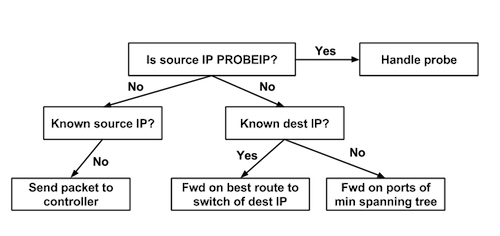
\includegraphics[scale=0.7]{IPLearner.png}
\caption{When a switch receives a packet with an unknown source IP, it sends it to the controller so that the controller can log the association between IP address and source switch, and update forwarding rules on switches appropriately.  If the destination IP address of a packet is known, it is routed according to best path rules determined by probing.  Otherwise, the packet is flooded on all ports in the minimum spanning tree.}
\end{figure}

Because SRON routes at the IP level, it must have a way of dynamically associating IP addresses with switches.  We achieve this in a way similar to how switches learn MAC-to-port mappings.  When a switch receives a packet with an unrecognized source IP address, it sends the packet to the controller.  If, for example, the incoming packet enters the network on $Switch_A$ and has IP 10.0.0.1, the controller logs this association.  It then examines all rules it has for routing between other switches in the network and $Switch_A$ (as determined by probing as described above).  The controller then updates all switches in the network to use this best path to route all packets with the destination IP address 10.0.0.1.  If, on the other hand, a switch receives a packet with an unknown destination IP, it sends the packet to an underlying mac learning module which forwards the packet to all ports along the network minimum spanning tree.  


\section{Implementation}
\subsection{Pyretic}
	We decided to build SRON in Pyretic\cite{pyretic}, a Python platform for programming SDNs.  Most major switch vendors support the OpenFlow API for programming switches, but writing OpenFlow messages directly is tedious, akin to programming in assembly. Pyretic sits above an OpenFlow controller platform (in our case, POX\cite{pox}), and allows programmers to write SDN programs in a high-level, modular way.  For example, consider the following excerpt from SRON that updates the network routing policy:\bigskip



\lstset{ %
language=Python,                % choose the language of the code
basicstyle=\ttfamily\scriptsize,
keywordstyle=\color{blue}\bfseries,
stringstyle=\color{red}\ttfamily,
commentstyle=\color{purple}\ttfamily,
showspaces=false,               % show spaces adding particular underscores
showstringspaces=false,         % underline spaces within strings
showtabs=false,                 % show tabs within strings adding particular underscores
frame=single,           % adds a frame around the code
tabsize=2,          % sets default tabsize to 2 spaces
captionpos=b,           % sets the caption-position to bottom
breaklines=true,        % sets automatic line breaking
breakatwhitespace=false,    % sets if automatic breaks should only happen at whitespace
escapeinside={\%*}{*)}          % if you want to add a comment within your code
}

	\begin{lstlisting}
	 def updatePolicy(self):
		print "Updating policy..."
		# probingPolicy explains how probes should be routed. self.query explains how the controller should log receieved probes
		probingPolicy = self.metricsPolicy + self.query

		# If a reRoutingPolicy has been created based on probe metrics, use it. Otherwise revert to a mac learner.
		if self.reRoutingPolicy:	
			self.policy = if_(match(srcip= PROBEIP), probingPolicy, self.reRoutingPolicy)
		else:
			self.policy = if_(match(srcip= PROBEIP), probingPolicy, self.macLearn)
	\end{lstlisting} 

We use the {\tt if\_({\it predicate}, policy1, policy2) } to indicate that all switches recieving a packet with source ip $PROBEIP$ should route that packet using {\tt probingPolicy}, which includes both forwarding that probe over all ports or dropping it (depending on whether the switch receiving this packet is the first or second hop on its path), as well as sending the packet up to the controller to be logged.  If the packet is not a probe packet, then it should either be routed via the {\tt reRoutingPolicy} or, if no such policy exists (for example, when the network is first brought up), should be routed via a simple mac learning module.  Note that rules in Pyretic are not written for individual switches.  Rather, rules for routing packets throughout the entire network are updated when the variable {\tt self.Policy} (where here the parent object is of type {\tt DynamicPolicy}) is updated.  Instructing only a particular switch to perform an action can be specified by creating a rule of the form: {\tt match(switch=someSwitch) >> somePolicy}.  Indeed Pyretic makes SDN programming concise. SRON is written only about 300 lines of Python.

\section{Evaluation}
\subsection{Experimental Setup}
Comparison with the mac learner module. We vary probe frequency, size of the network etc.
Using Harpoon, mininet.

\subsection{Results}
\subsection{Discussion}

\subsection{Future Work}

	It is difficult for any network simulation to capture all of the subtleties of real 
Internet traffic, and indeed our Mininet simulation of the Internet cannot give us 
full confidence that SRON will perform similarly when deployed when an ISP across the globe.
In the future, we would like to test SRON's performance when deployed on a PlanetLab\cite{planetlab} 
slice.  PlanetLab is a network of computers consisting of over 1090 nodes at 507 sites worldwide, 
which is designed for testing experimental network and distributed systems research projects.  With a 
virtual machine or ``slice'' of the PlanetLab network, we could test SRON across AS boundaries and with 
real network traffic, so that 
the difficult-to-predict decisions of BGP's policy-based routing could be compared with SRON.

As for making SRON ready for deployment, the current software design is closely tied to the original design of 
RON, which has since been improved upon in work by Nakao et al. \cite{Nakao:2006:SRO:1113361.1113372}, Gummadi et al.\cite{Gummadi:2004:IRI:1251254.1251267}, and more.  As mentioned in Section 2, this research has discovered techniques to reduce the amount of probing between nodes as well as ways to more intelligently use knowledge about the real network topology to design the overlay network topology.

\section{Conclusion}

\section{Acknowledgments}
This work would have been impossible without the constant guidance and feedback of Jennifer Rexford.


\bstctlcite{bstctl:etal, bstctl:nodash, bstctl:simpurl}
\bibliographystyle{IEEEtranS}
\bibliography{references}

\end{document}

